\chapter{La visión y el encéfalo}\label{ch:g11:vision-and-brain}

Tras un ictus, un paciente ve el mundo perfectamente --- en blanco,
negro y gris. Otro ve colores y formas pero ningún movimiento: un coche
está aquí y luego allí, sin nada en medio, y servir té es imposible
porque el chorro nunca parece moverse. Una tercera no reconoce las
caras, ni siquiera la suya en un espejo, aunque describe cada rasgo.
Sus \omterm{def:g11:the-eye:parts}{ojos} están intactos. Lo que cada uno ha perdido es una pieza del
encéfalo en la que se construye el ver. Este capítulo sigue al nervio
óptico dentro del encéfalo, cartografía lo que la \omterm{prop:g11:vision-and-brain:pathway}{corteza visual} hace
con las señales de la retina y muestra que ese mapa no es fijo: lo
construye la experiencia, lo modifica el aprendizaje y lo perturban las
drogas.

\section{De la retina a la corteza}

\begin{proposition}[La vía visual]\label{prop:g11:vision-and-brain:pathway}
El millón de fibras de cada nervio óptico va hacia atrás hasta el
\emph{quiasma óptico}, donde las fibras de la mitad nasal de cada
retina cruzan al otro lado mientras que las de la mitad temporal se
quedan en el suyo. Más allá del quiasma, cada \emph{tracto óptico}
lleva, por tanto, las señales de las mitades izquierdas de las dos
retinas (el tracto derecho) o de las mitades derechas (el izquierdo)
--- es decir, todo lo que se ve en una mitad del campo visual. Los
tractos hacen relevo en el \emph{tálamo} y llegan a la \emph{corteza
visual primaria}\index{corteza visual}, en la parte posterior de cada
hemisferio: el hemisferio izquierdo recibe la mitad derecha del campo
visual, y el derecho la mitad izquierda.
\end{proposition}
\begin{proof}[Pruebas experimentales]
Cortar un nervio óptico ciega un \omterm{def:g11:the-eye:parts}{ojo}; una lesión de un tracto óptico, o
de la \omterm{prop:g11:vision-and-brain:pathway}{corteza visual} de un hemisferio, deja los dos \omterm{def:g11:the-eye:parts}{ojos} funcionando
pero los ciega a los dos para la misma mitad del mundo --- la mitad
opuesta a la lesión. Estimular un punto de la \omterm{prop:g11:vision-and-brain:pathway}{corteza visual} de un
paciente despierto durante una operación le hace ver un destello en una
posición fija del campo; los puntos vecinos dan destellos vecinos: la
corteza contiene un mapa de la retina, y el centro del campo ocupa la
mayor parte de él.
\end{proof}

\begin{omfigure}
\begin{tikzpicture}[font=\small, >=Stealth, line cap=round]
  % top view: eyes at top, cortex at bottom
  \draw[thick, fill=omDef!8] (-2.2,4.2) circle (0.6); \draw[thick, fill=omDef!8] (2.2,4.2) circle (0.6);
  \node[anchor=south] at (-2.2,4.9) {ojo izquierdo}; \node[anchor=south] at (2.2,4.9) {ojo derecho};
  % visual field halves
  \node[omThm, anchor=east] at (-3.2,5.9) {campo izquierdo};
  \node[omMeth!60!black, anchor=west] at (3.2,5.9) {campo derecho};
  \draw[omThm, thick] (-4.4,5.6) -- (0,5.6); \draw[omMeth!60!black, thick] (0,5.6) -- (4.4,5.6);
  % fibres: left field falls on right halves of both retinas -> right hemisphere
  % from left eye: temporal half (left side of left eye) sees right field -> stays left; nasal half sees left field -> crosses
  \draw[thick, omMeth!60!black] (-2.7,3.7) -- (-2.7,1.6) -- (-1.2,0.3) -- (-1.2,-1.4);
  \draw[thick, omThm] (-1.7,3.7) -- (-1.7,1.6) -- (1.2,0.3) -- (1.2,-1.4);
  \draw[thick, omThm] (2.7,3.7) -- (2.7,1.6) -- (1.2,0.3);
  \draw[thick, omMeth!60!black] (1.7,3.7) -- (1.7,1.6) -- (-1.2,0.3);
  \fill (0,0.85) circle (2pt); \node[anchor=north] at (0,0.4) {quiasma óptico};
  % thalamus relays
  \draw[thick, fill=gray!20] (-1.2,-0.4) ellipse (0.35 and 0.25); \draw[thick, fill=gray!20] (1.2,-0.4) ellipse (0.35 and 0.25);
  \node[anchor=east] at (-1.6,-0.4) {tálamo};
  % cortex
  \draw[thick, fill=omMeth!15] (-2.4,-2.6) rectangle (-0.2,-1.4); \draw[thick, fill=omThm!15] (0.2,-2.6) rectangle (2.4,-1.4);
  \node[align=center] at (-1.3,-2.0) {corteza visual\\ izquierda}; \node[align=center] at (1.3,-2.0) {corteza visual\\ derecha};
  \node[anchor=north, align=center, font=\scriptsize] at (-1.3,-2.7) {ve el campo\\ derecho};
  \node[anchor=north, align=center, font=\scriptsize] at (1.3,-2.7) {ve el campo\\ izquierdo};
  \node[anchor=west, align=left, font=\scriptsize] at (3.0,2.6) {nervios ópticos:\\ uno por ojo};
  \node[anchor=west, align=left, font=\scriptsize] at (3.0,0.0) {tractos ópticos:\\ uno por medio campo};
\end{tikzpicture}

{\small La vía visual vista desde arriba. La luz de la mitad izquierda
del campo (rojo) cae sobre la mitad derecha de cada retina; esas
fibras, cruzando en el quiasma cuando hace falta, se agrupan en el
tracto óptico derecho y llegan a la \omterm{prop:g11:vision-and-brain:pathway}{corteza visual} derecha. Cada
hemisferio ve la mitad opuesta del mundo con los dos \omterm{def:g11:the-eye:parts}{ojos}.}
\end{omfigure}

\begin{omfigure}
\begin{tikzpicture}
  \node[anchor=south west, inner sep=0] (img) at (0,0)
    {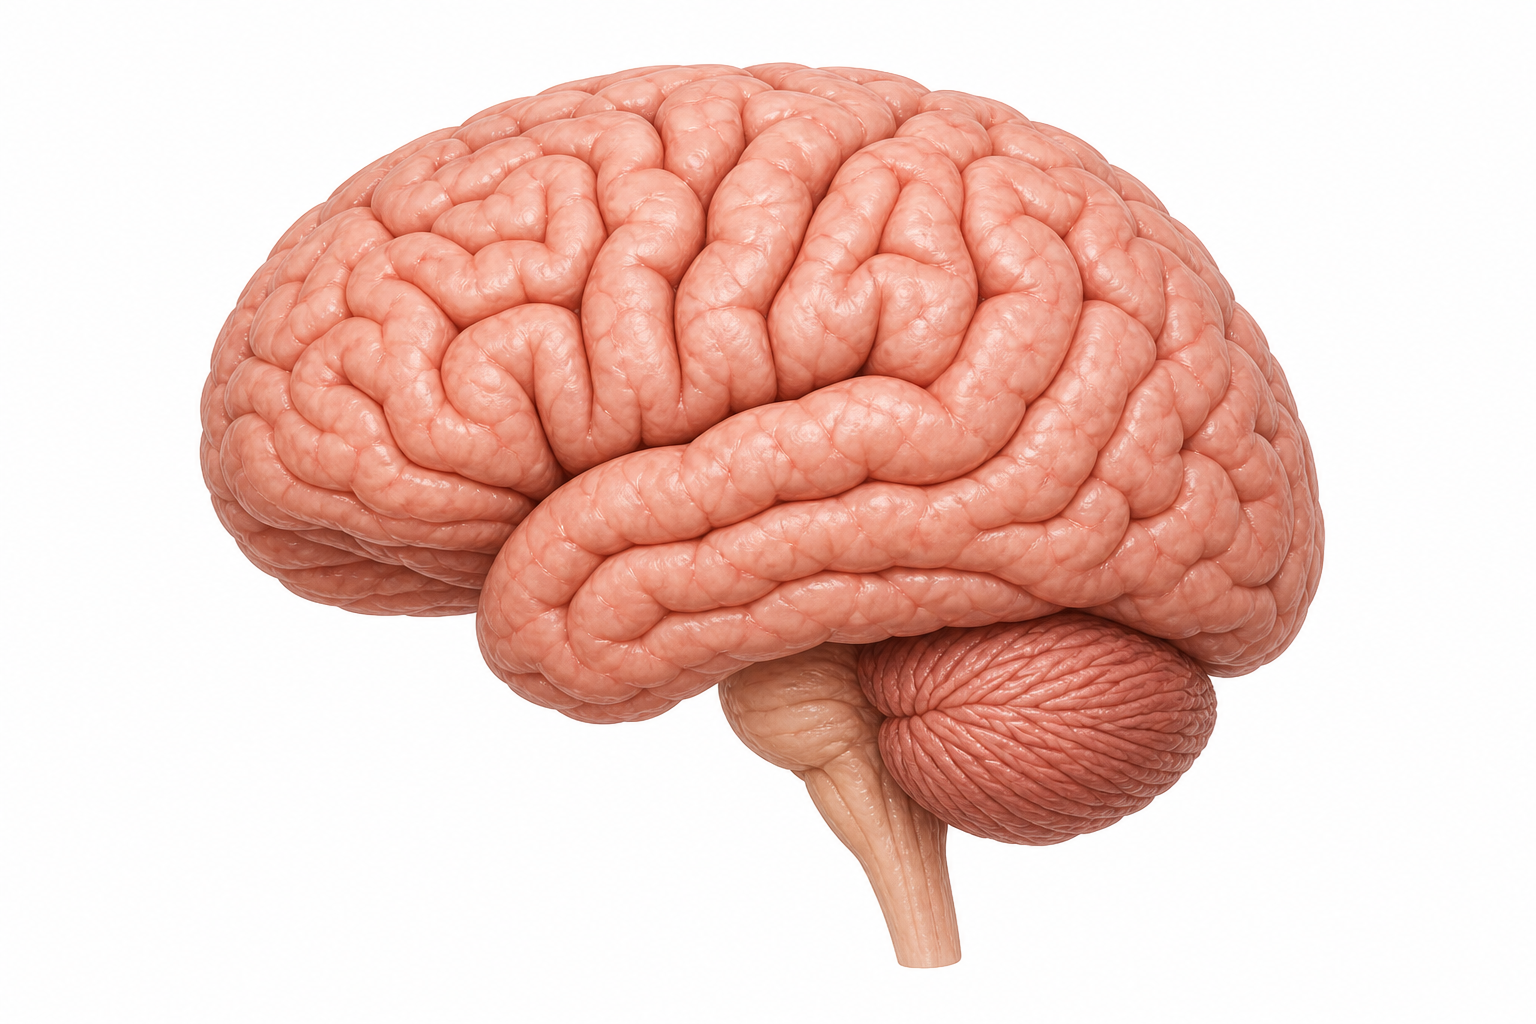
\includegraphics[width=0.52\linewidth]{images/book2/ai/fig-brain-side.png}};
  \begin{scope}[x={(img.south east)}, y={(img.north west)},
      every node/.style={font=\small}]
    \draw[omDef, thick] (0.85,0.55) -- (1.05,0.70) node[right, align=left] {corteza visual primaria\\ (lóbulo occipital)};
    \draw[omDef, thick] (0.70,0.75) -- (0.80,1.06) node[above] {lóbulo parietal};
    \draw[omDef, thick] (0.28,0.72) -- (0.20,1.06) node[above] {lóbulo frontal};
    \draw[omDef, thick] (0.48,0.42) -- (0.40,-0.06) node[below] {lóbulo temporal};
    \draw[omDef, thick] (0.70,0.28) -- (1.05,0.20) node[right] {cerebelo};
  \end{scope}
\end{tikzpicture}

{\small El encéfalo visto desde el lado izquierdo. La \omterm{prop:g11:vision-and-brain:pathway}{corteza visual
primaria} está en la parte más posterior, en el lóbulo occipital; las
demás áreas visuales se extienden hacia delante desde ella, hacia el
lóbulo temporal (qué son las cosas) y el lóbulo parietal (dónde están y
cómo se mueven).}
\end{omfigure}

\section{Muchas áreas, una sola percepción}

\begin{proposition}[Áreas visuales especializadas]\label{prop:g11:vision-and-brain:areas}
La \omterm{prop:g11:vision-and-brain:pathway}{corteza visual primaria} pasa su análisis a una docena de
\emph{áreas visuales} más, cada una especializada: una extrae el color,
otra el movimiento, y otras la forma, la profundidad, las caras, las
palabras escritas. Sus resultados se combinan --- con la memoria, con
los demás sentidos --- en la percepción única y coherente que
experimentamos. La percepción es una construcción: el encéfalo rellena
el punto ciego, completa los contornos ocultos, mantiene constantes los
colores bajo luces cambiantes y puede ser engañado por ilusiones que
explotan sus reglas.
\end{proposition}
\begin{proof}[Pruebas experimentales]
Las lesiones localizadas disocian los componentes: un paciente con daño
en el área del color ve un mundo en gris con agudeza normal; el daño en
el área del movimiento deja intactos el color y la forma pero suprime
la percepción del movimiento; el daño en una región del lóbulo temporal
suprime solo el reconocimiento de las caras. Las imágenes funcionales
de voluntarios sanos muestran que se encienden esas mismas áreas, una
con los patrones de color, otra con puntos en movimiento y otra con
caras, mientras que la corteza primaria responde a todo. Los electrodos
en animales encuentran, en cada área, neuronas que responden al rasgo
de esa área y a poco más.
\end{proof}

\begin{omfigure}
\begin{tikzpicture}[font=\small, >=Stealth,
  b/.style={draw, rounded corners, align=center, text width=2.5cm, minimum height=1.0cm}]
  \node[b, fill=omDef!12] (ret) at (0,0) {retina:\\ de la luz a las señales};
  \node[b, fill=omDef!12] (v1) at (3.6,0) {corteza visual\\ primaria: bordes,\\ orientaciones, mapa};
  \node[b, fill=omProp!15] (col) at (7.4,1.6) {área del color};
  \node[b, fill=omProp!15] (mov) at (7.4,0) {área del movimiento};
  \node[b, fill=omProp!15] (shp) at (7.4,-1.6) {áreas de la forma\\ y de las caras};
  \node[b, fill=omMeth!15, text width=2.8cm] (per) at (11.2,0) {percepción:\\ una escena, con\\ la memoria añadida};
  \draw[->, thick] (ret) -- (v1);
  \draw[->, thick] (v1) -- (col); \draw[->, thick] (v1) -- (mov); \draw[->, thick] (v1) -- (shp);
  \draw[->, thick] (col) -- (per); \draw[->, thick] (mov) -- (per); \draw[->, thick] (shp) -- (per);
\end{tikzpicture}

{\small De las señales a una escena. La corteza primaria reparte su
análisis entre áreas especializadas cuyos resultados se recombinan. Una
lesión en un área retira un atributo --- el color, el movimiento, las
caras --- y deja el resto.}
\end{omfigure}

\begin{example}[Tres pacientes, tres áreas]\label{ex:g11:vision-and-brain:patients}
La paciente que ve en gris tiene una lesión del área del color en los
dos lados; los \omterm{def:g11:the-eye:photoreceptors}{conos} de su retina funcionan, y su corteza primaria
recibe sus señales, pero ha desaparecido la etapa que convierte las
proporciones de los \omterm{def:g11:the-eye:photoreceptors}{conos} en color. La paciente que no ve el movimiento
ha perdido el área del movimiento: ve instantáneas sucesivas. La
paciente que no reconoce las caras tiene una lesión del área de las
caras del lóbulo temporal; reconoce a las personas por la voz o por un
sombrero. En cada caso lo que se pierde es preciso, y lo que queda
muestra que las demás áreas trabajan por su cuenta.
\end{example}

\section{Una corteza construida por la experiencia}

\begin{proposition}[La plasticidad]\label{prop:g11:vision-and-brain:plasticity}
Las conexiones de la \omterm{prop:g11:vision-and-brain:pathway}{corteza visual} no están fijadas al nacer. Durante
un \emph{periodo crítico} de la primera etapa de la vida las modela lo
que ven los \omterm{def:g11:the-eye:parts}{ojos}; en el adulto siguen cambiando, más despacio, con el
aprendizaje y con el uso. Esta \emph{plasticidad
cerebral}\index{plasticidad cerebral} es una propiedad de las neuronas:
las conexiones que se usan se refuerzan y se multiplican, y las que no
se debilitan y se podan.
\end{proposition}
\begin{proof}[Pruebas experimentales]
Hubel y Wiesel (en los años sesenta) registraron la \omterm{prop:g11:vision-and-brain:pathway}{corteza visual} de
gatos y de monos. En un animal normal, casi todas las neuronas
responden a los dos \omterm{def:g11:the-eye:parts}{ojos}. En un animal al que se le mantuvo cerrado un
\omterm{def:g11:the-eye:parts}{ojo} durante sus primeros meses, casi todas las neuronas responden solo
al \omterm{def:g11:the-eye:parts}{ojo} abierto: las conexiones del \omterm{def:g11:the-eye:parts}{ojo} cerrado han sido ocupadas.
Cerrar el \omterm{def:g11:the-eye:parts}{ojo} de un adulto durante ese mismo tiempo no cambia nada. En
los humanos, un niño con un \omterm{def:g11:the-eye:parts}{ojo} muy desenfocado o desviado que no se
corrige antes de los siete años aproximadamente conserva un \omterm{def:g11:the-eye:parts}{ojo} débil
para siempre --- la ambliopía ---, por buena que sea después su
óptica. En los adultos, aprender a leer braille agranda el área
cortical dedicada al dedo que lee; aprender malabares agranda las áreas
que procesan el movimiento, y vuelven a encogerse si se deja de
practicar.
\end{proof}

\begin{omfigure}
\begin{tikzpicture}
\begin{axis}[
  ybar, bar width=9pt,
  width=0.86\linewidth, height=5.6cm,
  axis x line=bottom, axis y line=left,
  ymin=0, ymax=60, ylabel={neuronas corticales (\%)},
  ylabel style={font=\small},
  symbolic x coords={solo ojo izq., sobre todo izq., los dos por igual, sobre todo der., solo ojo der.},
  xtick=data, tick label style={font=\small},
  xlabel={qué ojo activa la neurona},
  xlabel style={font=\small, at={(axis description cs:0.5,-0.16)}, anchor=north},
  enlarge x limits=0.15, ytick={0,20,40,60},
  legend style={at={(0.5,-0.34)}, anchor=north, legend columns=2, font=\small, draw=none},
]
\addplot[fill=omDef!50, draw=omDef] coordinates {(solo ojo izq.,12) (sobre todo izq.,20) (los dos por igual,36) (sobre todo der.,20) (solo ojo der.,12)};
\addplot[fill=omThm!50, draw=omThm] coordinates {(solo ojo izq.,2) (sobre todo izq.,3) (los dos por igual,5) (sobre todo der.,30) (solo ojo der.,60)};
\legend{gatito normal, gatito con el ojo izquierdo cerrado tres meses}
\end{axis}
\end{tikzpicture}

{\small El hallazgo de Hubel y Wiesel, redondeado. En un gatito normal,
casi todas las neuronas de la \omterm{prop:g11:vision-and-brain:pathway}{corteza visual} responden a los dos \omterm{def:g11:the-eye:parts}{ojos}.
Tras tres meses con el \omterm{def:g11:the-eye:parts}{ojo} izquierdo cerrado, nueve de cada diez
neuronas responden solo al \omterm{def:g11:the-eye:parts}{ojo} derecho: se han perdido las conexiones
del \omterm{def:g11:the-eye:parts}{ojo} sin usar.}
\end{omfigure}

\begin{example}[Por qué el estrabismo debe tratarse pronto]\label{ex:g11:vision-and-brain:amblyopia}
Un niño de tres años con un \omterm{def:g11:the-eye:parts}{ojo} desviado hacia dentro ve doble, y el
encéfalo suprime la imagen más débil. Si no se endereza el \omterm{def:g11:the-eye:parts}{ojo}, o no se
tapa el \omterm{def:g11:the-eye:parts}{ojo} bueno unas horas al día para obligar a trabajar al débil,
la corteza se reorganiza en torno al \omterm{def:g11:the-eye:parts}{ojo} bueno durante el periodo
crítico y el \omterm{def:g11:the-eye:parts}{ojo} débil, aunque ópticamente sea perfecto, queda ciego al
detalle fino de por vida. Tratado a los tres años, el niño recupera la
visión completa; tratado a los doce, casi nada.
\end{example}

\section{Las drogas y el encéfalo que ve}

\begin{proposition}[Neuronas, mensajeros y moléculas que los imitan]\label{prop:g11:vision-and-brain:drugs}
Las neuronas se comunican en las \emph{sinapsis} liberando mensajeros
químicos, los \emph{neurotransmisores}, sobre los receptores de la
\omterm{def:g10:cells-common-unit:cell}{célula} siguiente; el último año describe el mecanismo. Varios
neurotransmisores, entre ellos la \emph{serotonina}, regulan el paso de
las señales por las áreas visuales. Las moléculas cuya forma se parece
a la de un neurotransmisor pueden unirse a sus receptores y perturbar
ese paso: la dietilamida del ácido lisérgico (LSD) se une a los
receptores de serotonina de la \omterm{prop:g11:vision-and-brain:pathway}{corteza visual} y produce alucinaciones
--- colores, formas y movimientos vistos sin ninguna luz que les
corresponda. Estas drogas pueden dejar cambios duraderos: episodios que
reaparecen meses después y, en algunas personas, alteraciones visuales
persistentes.
\end{proposition}
\admitted

\begin{example}[Lo que muestra una alucinación]\label{ex:g11:vision-and-brain:hallucination}
Bajo el LSD, la retina no cambia y la corteza primaria sigue
cartografiando lo que ven los \omterm{def:g11:the-eye:parts}{ojos}; la perturbación está en las áreas
posteriores y en cómo se combinan. Aparecen patrones que se parecen a
las piezas de construcción de la propia corteza --- rejillas,
espirales, túneles --- porque la droga pone en marcha la maquinaria de
la percepción sin su entrada. La alucinación es una demostración, por
avería, de que el ver lo hace el encéfalo y de que una molécula puede
cambiarlo.
\end{example}

\begin{method}[Localizar un déficit visual]\label{met:g11:vision-and-brain:locate}
\begin{enumerate}
  \item Un \omterm{def:g11:the-eye:parts}{ojo} ciego y el otro normal: el \omterm{def:g11:the-eye:parts}{ojo} o su nervio óptico, antes
        del quiasma.
  \item Los dos \omterm{def:g11:the-eye:parts}{ojos} ciegos para la misma mitad del campo: el tracto
        óptico, el tálamo o la corteza primaria del lado opuesto.
  \item Los dos \omterm{def:g11:the-eye:parts}{ojos} ciegos para las mitades externas del campo: el
        quiasma, donde se cortan las fibras que cruzan.
  \item Visión intacta pero con un atributo perdido (color, movimiento,
        caras): el área especializada correspondiente.
  \item Percepción alterada con los \omterm{def:g11:the-eye:parts}{ojos} y la corteza normales y de
        forma pasajera: una droga o una causa metabólica.
\end{enumerate}
\end{method}

\begin{remark}[Lo que ha mostrado este año]\label{rem:g11:vision-and-brain:year}
El \omterm{def:g11:the-eye:parts}{ojo} del \cref{ch:g11:the-eye} era cuestión de \omterm{def:g10:universal-dna:gene}{genes} y de \omterm{def:g10:chemistry-of-life:families}{proteínas}:
\omterm{def:g11:the-eye:photoreceptors}{opsinas}, sus duplicaciones, un daltonismo heredado en el X. El encéfalo
de este capítulo es cuestión de conexiones, modeladas por el uso. Entre
ambos está todo el asunto del año --- de la secuencia de un \omterm{def:g10:universal-dna:gene}{gen} a un
rasgo, y del rasgo a lo que una persona puede hacer --- y la lección de
que en cada paso el \omterm{def:g11:enzymes-and-phenotype:phenotype}{genotipo} propone y el ambiente, desde la
temperatura de las orejas de un gato hasta la luz que recibe el \omterm{def:g11:the-eye:parts}{ojo} de
un gatito, dispone.
\end{remark}

\section{Ejercicios}

\begin{exercise}[$\star$]\label{exo:g11:vision-and-brain:1}
Sigue el camino de una señal desde la mitad izquierda del campo visual
hasta la corteza.
\end{exercise}

\begin{exercise}[$\star$]\label{exo:g11:vision-and-brain:2}
¿Qué ocurre en el quiasma óptico, y qué fibras cruzan?
\end{exercise}

\begin{exercise}[$\star$]\label{exo:g11:vision-and-brain:3}
Nombra tres áreas visuales especializadas y el déficit que produce una
lesión de cada una.
\end{exercise}

\begin{exercise}[$\star$]\label{exo:g11:vision-and-brain:4}
Define la \omterm{prop:g11:vision-and-brain:plasticity}{plasticidad cerebral} y el periodo crítico.
\end{exercise}

\begin{exercise}[$\star$]\label{exo:g11:vision-and-brain:5}
¿Cómo actúa el LSD sobre el sistema visual?
\end{exercise}

\begin{exercise}[$\star\star$]\label{exo:g11:vision-and-brain:6}
Con el \cref{met:g11:vision-and-brain:locate}, localiza la lesión de un
paciente ciego para la mitad derecha del campo con los dos \omterm{def:g11:the-eye:parts}{ojos}.
\end{exercise}

\begin{exercise}[$\star\star$]\label{exo:g11:vision-and-brain:7}
Un \omterm{def:g11:cancer:cancer}{tumor} presiona el quiasma óptico desde abajo y corta las fibras que
cruzan. ¿Qué partes del campo pierde el paciente? Explícalo con la
figura.
\end{exercise}

\begin{exercise}[$\star\star$]\label{exo:g11:vision-and-brain:8}
En la figura de Hubel y Wiesel, ¿qué fracción de las neuronas responde
en alguna medida al \omterm{def:g11:the-eye:parts}{ojo} izquierdo en el gatito normal y en el privado?
\end{exercise}

\begin{exercise}[$\star\star$]\label{exo:g11:vision-and-brain:9}
¿Por qué tapar el \omterm{def:g11:the-eye:parts}{ojo} bueno de un niño con estrabismo unas horas al día
trata la ambliopía? ¿Por qué el mismo tratamiento fracasa en un adulto?
\end{exercise}

\begin{exercise}[$\star\star$]\label{exo:g11:vision-and-brain:10}
Explica por qué la paciente que ve en gris no es daltónica en el
sentido del \cref{ch:g11:the-eye}, y cómo podría distinguir una prueba
las dos condiciones.
\end{exercise}

\begin{exercise}[$\star\star$]\label{exo:g11:vision-and-brain:11}
El área cortical de los dedos de una pianista es mayor que la media.
Explícalo con la plasticidad y di qué predices si deja de tocar durante
años.
\end{exercise}

\begin{exercise}[$\star\star\star$]\label{exo:g11:vision-and-brain:12}
Una persona ciega de nacimiento por cataratas se las hace quitar a los
30. Predice qué ve en las primeras semanas y qué recuperará y qué no,
usando el periodo crítico.
\end{exercise}

\begin{exercise}[$\star\star\star$]\label{exo:g11:vision-and-brain:13}
Explica por qué el mapa cortical dedica más superficie al centro del
campo que a la periferia, usando el reparto de receptores y de \omterm{def:g10:cells-common-unit:cell}{células}
ganglionares del \cref{ch:g11:the-eye}.
\end{exercise}

\begin{exercise}[$\star\star\star$]\label{exo:g11:vision-and-brain:14}
Las imágenes funcionales muestran el área del color activa cuando una
persona imagina una manzana roja con los \omterm{def:g11:the-eye:parts}{ojos} cerrados. ¿Qué dice eso
sobre la relación entre las áreas especializadas y la percepción, y
sobre las alucinaciones?
\end{exercise}

\begin{exercise}[$\star\star\star$]\label{exo:g11:vision-and-brain:15}
``Ver lo hace el \omterm{def:g11:the-eye:parts}{ojo}.'' Reescribe correctamente esta afirmación en un
párrafo, usando los tres pacientes, los gatitos y la droga.
\end{exercise}

\section{Problema: Cuatro pacientes y un gatito}

\begin{problem}[{Problema de fin de semana --- déficits visuales
localizados a lo largo de la vía, una corteza cartografiada por
estimulación, la privación de un gatito contada y el estrabismo de un
niño tratado a tiempo}]
\label{pb:g11:vision-and-brain:1}
Se examina a cuatro pacientes. A: ciego del \omterm{def:g11:the-eye:parts}{ojo} izquierdo, con el
derecho normal. B: los dos \omterm{def:g11:the-eye:parts}{ojos} ciegos para la mitad izquierda del
campo. C: los dos \omterm{def:g11:the-eye:parts}{ojos} ciegos para la mitad externa de su campo (el \omterm{def:g11:the-eye:parts}{ojo}
izquierdo para la izquierda y el derecho para la derecha). D: campos
normales y agudeza normal, pero no percibe el movimiento.

\medskip
\noindent\textbf{Parte I --- Localizar.}
\begin{enumerate}
  \item Localiza la lesión de A. ¿Qué estructura, y antes o después del
        quiasma?
  \item Localiza la lesión de B y di por qué tiene que estar después
        del quiasma.
  \item Localiza con precisión la lesión de C y explica qué fibras
        quedan cortadas.
  \item Localiza la lesión de D. ¿Qué te dice sobre la corteza primaria
        el hecho de que se conserven los campos y la agudeza?
  \item Para cada paciente, di si la retina está intacta y cómo lo
        comprobarías.
\end{enumerate}

\medskip
\noindent\textbf{Parte II --- El mapa.}
Durante una operación, estimular puntos de la \omterm{prop:g11:vision-and-brain:pathway}{corteza visual} derecha de
un paciente produce destellos. Estimular la punta del lóbulo occipital
da un destello en el centro del campo; los puntos más hacia delante dan
destellos más hacia fuera del campo izquierdo; \qty{1}{cm} de corteza
en la punta cubre unos $2^\circ$ del campo, mientras que \qty{1}{cm}
más hacia delante cubre $20^\circ$.
\begin{enumerate}[resume]
  \item ¿Por qué están todos los destellos en el campo izquierdo?
  \item ¿Cuánta corteza representa los $2^\circ$ centrales frente a una
        banda de $2^\circ$ situada a $40^\circ$ del centro? Calcula el
        cociente.
  \item Relaciona ese cociente con la fóvea y la periferia de la
        retina.
  \item Una lesión pequeña en la punta del lóbulo occipital derecho:
        ¿qué pierde el paciente? ¿Y una lesión del mismo tamaño más
        hacia delante?
  \item ¿Por qué el paciente con la lesión central pequeña todavía
        puede leer, despacio, moviendo los \omterm{def:g11:the-eye:parts}{ojos}?
\end{enumerate}

\medskip
\noindent\textbf{Parte III --- El gatito.}
A partir de la figura de Hubel y Wiesel.
\begin{enumerate}[resume]
  \item En el gatito normal, ¿qué porcentaje de neuronas responden en
        alguna medida a los dos \omterm{def:g11:the-eye:parts}{ojos}?
  \item En el gatito privado, ¿qué porcentaje responden de algún modo
        al \omterm{def:g11:the-eye:parts}{ojo} cerrado (el izquierdo)?
  \item La retina y el nervio óptico del \omterm{def:g11:the-eye:parts}{ojo} cerrado están intactos.
        ¿Adónde ha ido su entrada y qué ha ocupado el sitio?
  \item El mismo cierre en un gato adulto no cambia nada. ¿Qué
        establece eso y cuál es su equivalente humano?
  \item A un gatito se le cierran los dos \omterm{def:g11:the-eye:parts}{ojos} durante tres meses.
        Predice el histograma y la visión del animal después.
\end{enumerate}

\medskip
\noindent\textbf{Parte IV --- El niño.}
Un niño de cuatro años tiene el \omterm{def:g11:the-eye:parts}{ojo} izquierdo desviado hacia dentro; su
óptica es normal. Sin tratamiento, la corteza pasa a ocuparse de la
entrada del \omterm{def:g11:the-eye:parts}{ojo} derecho.
\begin{enumerate}[resume]
  \item Explica, con el gatito, qué le ocurrirá a la visión del \omterm{def:g11:the-eye:parts}{ojo}
        izquierdo si no se hace nada, y por qué las gafas solas no lo
        impedirán.
  \item El tratamiento consiste en tapar el \omterm{def:g11:the-eye:parts}{ojo} \emph{derecho} varias
        horas al día durante meses. Explica por qué se tapa el \omterm{def:g11:the-eye:parts}{ojo}
        bueno.
  \item ¿Por qué hay que hacerlo antes de los siete años
        aproximadamente, y por qué fracasa el mismo tratamiento a los
        quince?
  \item Un adulto que pierde un \omterm{def:g11:the-eye:parts}{ojo} a los treinta no pierde de la misma
        manera la corteza que le estaba dedicada. Concilia esto con el
        gatito.
  \item Enuncia el resultado: las cuatro lesiones localizadas de
        delante atrás de la vía, y la única propiedad de la corteza ---
        con su nombre --- que hace que el tratamiento del niño solo
        funcione a tiempo.
\end{enumerate}
\end{problem}
